\documentclass[aspectratio=169,9pt]{beamer}

\usepackage[utf8]{inputenc}
\usepackage[T1]{fontenc}
\usepackage{mathptmx}
\usepackage[scaled=0.92]{helvet}
\usepackage{graphicx}
\usepackage{xcolor}
\usepackage{tikz}
\usetikzlibrary{positioning,arrows.meta,calc}
\usepackage{booktabs}
\usepackage{array}
\usepackage{tabularx}
\usepackage{colortbl}
\usepackage{microtype}

% Exact Palette from Reference PPTX (7181xxxxxxx.pptx - Elegant Bachelor Thesis)
\definecolor{refFrame}{HTML}{CFDEE7}   % lt1: outer sky-slate border & star accent
\definecolor{refPage}{HTML}{FAFAFA}    % lt2: crisp off-white inner slide canvas
\definecolor{refInk}{HTML}{45474A}     % dk1 (slightly deepened from 5C5C5F for print/projector clarity)
\definecolor{refSlate}{HTML}{809FAF}   % dk2: slate-blue accent & slide number
\definecolor{refSoft}{HTML}{EDF3F7}    % light tint for cards & zebra rows
\definecolor{refBorder}{HTML}{C4D6E1}  % subtle card/table border
\definecolor{refRed}{HTML}{CC0000}     % reference Slide 1 student/guide accent

\usetheme{default}
\usecolortheme{default}
\usefonttheme{serif}
\setbeamertemplate{navigation symbols}{}
\setbeamersize{text margin left=1.05cm, text margin right=1.05cm}

\setbeamercolor{normal text}{fg=refInk,bg=refFrame}
\setbeamercolor{structure}{fg=refInk}
\setbeamercolor{frametitle}{fg=refInk,bg=refPage}
\setbeamercolor{itemize item}{fg=refSlate}
\setbeamercolor{itemize subitem}{fg=refSlate}

\setbeamertemplate{itemize item}{\raisebox{0.18ex}{\tiny$\bullet$}}
\setbeamertemplate{itemize subitem}{\small--}

% Reference Slidesgo Canvas: #CFDEE7 outer border + #FAFAFA inner page + subtle 4-point star
\setbeamertemplate{background}{%
  \begin{tikzpicture}[remember picture, overlay]
    % Outer pale slate-blue frame
    \fill[refFrame] (current page.south west) rectangle (current page.north east);
    % Inner off-white card (matches reference 0.213in / 0.217in inset)
    \fill[refPage] ([xshift=0.26cm,yshift=0.26cm]current page.south west)
      rectangle ([xshift=-0.26cm,yshift=-0.26cm]current page.north east);
    % Top-center subtle 4-point star on content slides (exact slideLayout2 star4)
    \ifnum\theframenumber>1\relax%
      \coordinate (sc) at ([yshift=-0.54cm]current page.north);
      \draw[refFrame, line width=0.9pt]
        ($(sc)+(0,0.18cm)$) -- ($(sc)+(0.045cm,0.045cm)$)
        -- ($(sc)+(0.18cm,0)$) -- ($(sc)+(0.045cm,-0.045cm)$)
        -- ($(sc)+(0,-0.18cm)$) -- ($(sc)+(-0.045cm,-0.045cm)$)
        -- ($(sc)+(-0.18cm,0)$) -- ($(sc)+(-0.045cm,0.045cm)$) -- cycle;
    \fi%
  \end{tikzpicture}%
}

% Reference Content Header: Clean Bold ALL-CAPS Times New Roman Title
\setbeamertemplate{frametitle}{%
  \vspace*{0.44cm}%
  \noindent{\Large\bfseries\color{refInk}\insertframetitle}\par%
  \vspace{0.06cm}%
  \noindent\textcolor{refFrame}{\rule{\textwidth}{0.9pt}}\par%
  \vspace{0.08cm}%
}

% Reference Minimal Footer: Centered Slide Number Only (No College/Company Text)
\setbeamertemplate{footline}{%
  \ifnum\theframenumber>1\relax%
  \begin{beamercolorbox}[wd=\paperwidth,ht=0.42cm,dp=0.28cm]{}%
    \centering{\scriptsize\color{refSlate}\insertframenumber}%
  \end{beamercolorbox}%
  \fi%
}

% Clean Light Slate Card Helper
\newcommand{\refcard}[2]{%
  \begin{tikzpicture}
    \node[
      draw=refBorder,
      fill=refSoft,
      rounded corners=3pt,
      line width=0.6pt,
      inner sep=8pt,
      text width=\dimexpr\linewidth-18pt\relax,
      align=left
    ] {%
      \raggedright\hyphenpenalty=10000\exhyphenpenalty=10000
      {\normalsize\bfseries\color{refInk}#1}\par\vspace{3pt}%
      {\small\color{refInk}#2}%
    };
  \end{tikzpicture}%
}

\begin{document}

% =====================================================================
% SLIDE 1: TITLE SLIDE (Exact 7181xxxxxxx.pptx Layout)
% =====================================================================
\begin{frame}[plain]
\vspace*{0.30cm}
\noindent
\begin{minipage}[c]{0.72\linewidth}
  
\includegraphics[height=1.22cm]{assets/srec_logo.png}
\end{minipage}\hfill
\begin{minipage}[c]{0.22\linewidth}
  \raggedleft
  
\includegraphics[height=1.24cm]{assets/snr_logo.png}
\end{minipage}

\vspace{0.34cm}
\begin{center}
  {\normalsize\sffamily\bfseries\color{refInk}DEPARTMENT OF M.Tech COMPUTER SCIENCE \& ENGINEERING}\\[2pt]
  {\small\sffamily\bfseries\color{refInk}(5 Years Integrated Programme)}

  \vspace{0.58cm}
  {\LARGE\bfseries\color{refInk}INTERNSHIP REVIEW 3}\\[6pt]
  {\Large\bfseries\color{refInk}Project Title: Voice-Controlled Hands-Free Browser Automation}\\[4pt]
  {\normalsize\color{refSlate}Accessible Web Surfing in Google Chrome for Physically Challenged Users}
\end{center}

\vspace{0.85cm}
\noindent
\begin{minipage}[t]{0.46\linewidth}
  {\normalsize\bfseries\color{refInk}GUIDE NAME:}\\[3pt]
  {\normalsize\color{refRed}Mrs. NISHANTHI AP/CSE}
\end{minipage}\hfill
\begin{minipage}[t]{0.46\linewidth}
  \raggedleft
  {\normalsize\bfseries\color{refInk}BY:}\\[3pt]
  {\normalsize\color{refRed}ABISHEK S (71812353005)}
\end{minipage}
\end{frame}

% =====================================================================
% SLIDE 2: COMPANY DETAILS
% =====================================================================
\begin{frame}{COMPANY DETAILS}
\begin{columns}[T,totalwidth=\textwidth]
  \begin{column}{0.58\textwidth}
    {\large\bfseries\color{refInk}LANGFORDPOWERTECH}\\[5pt]
    {\small\color{refInk}\raggedright
    LangfordPowerTech is a software and AI development company delivering practical AI applications, freelance engineering projects, and dependable solutions for partner and vendor organizations.}

    \vspace{0.26cm}
    \begin{itemize}\setlength{\itemsep}{6pt}\small
      \item \textbf{AI \& Custom Development:} Builds practical AI applications and developer solutions tailored to real-world workflows.
      \item \textbf{Freelance \& Client Projects:} Delivers end-to-end software projects with reliable turnaround and strong engineering quality.
      \item \textbf{Partner \& Vendor Solutions:} Collaborates with partner and vendor companies to ship scalable digital products across domains.
      \item \textbf{Final-Year Project Guidance:} Mentors college students on industry-grade projects solving practical accessibility and business needs.
    \end{itemize}
  \end{column}
  \begin{column}{0.38\textwidth}
    \refcard{Core Focus Areas}{%
      \textbullet\ AI Application Development\\[4pt]
      \textbullet\ Freelance \& Custom Engineering\\[4pt]
      \textbullet\ Partner \& Vendor Delivery\\[4pt]
      \textbullet\ Final-Year Project Mentorship
    }\par\vspace{0.24cm}
    \refcard{Confidentiality Scope}{%
      Under company NDA policy, this review presents the \textbf{problem, spoken inputs, browser outputs, and verified results} without disclosing proprietary internal architecture.
    }
  \end{column}
\end{columns}
\end{frame}

% =====================================================================
% SLIDE 3: PROJECT OVERVIEW & OBJECTIVES
% =====================================================================
\begin{frame}{PROJECT OVERVIEW \& OBJECTIVES}
\begin{columns}[T,totalwidth=\textwidth]
  \begin{column}{0.52\textwidth}
    {\footnotesize\bfseries\color{refSlate}PROJECT TITLE}\\[2pt]
    {\large\bfseries\color{refInk}Voice-Controlled Hands-Free Browser Automation}

    \vspace{0.30cm}
    {\footnotesize\bfseries\color{refSlate}OVERVIEW}\\[2pt]
    {\small\color{refInk}\raggedright
    Everyday life---education, news, video lectures, documents, and online services---depends on web browsers. This project enables people who cannot use a mouse or keyboard to surf regular \textbf{Google Chrome} independently using natural spoken voice alone.}

    \vspace{0.30cm}
    {\footnotesize\bfseries\color{refSlate}TARGET USERS}\\[2pt]
    {\small\color{refInk}\raggedright
    Individuals with upper-limb or motor disabilities, elderly users, and anyone needing safe, hands-free web access.}
  \end{column}
  \begin{column}{0.44\textwidth}
    \refcard{Core Objectives}{%
      \textbf{1. Full Hands-Free Surfing:} Open sites, search, click, scroll, read pages, and manage tabs in Chrome by voice.\\[6pt]
      \textbf{2. Natural Spoken Phrases:} Respond to everyday speech rather than rigid commands or keyboard shortcuts.\\[6pt]
      \textbf{3. Safe User Control:} Pause and request verbal approval before sensitive actions.\\[6pt]
      \textbf{4. Reliable Daily Use:} Keep Chrome open, responsive, and resilient across long sessions.
    }
  \end{column}
\end{columns}
\end{frame}

% =====================================================================
% SLIDE 4: PROBLEM DEFINITION
% =====================================================================
\begin{frame}{PROBLEM DEFINITION}
{\small\color{refInk}\raggedright
Standard browsers like Google Chrome assume precise \textbf{mouse pointing, clicking, scrolling, and keyboard typing}. For people with upper-limb disabilities, paralysis, arthritis, or motor impairments, everyday web browsing is slow, exhausting, or completely inaccessible.}

\vspace{0.32cm}
\begin{columns}[T,totalwidth=\textwidth]
  \begin{column}{0.48\textwidth}
    \refcard{Gaps in Existing Approaches}{%
      \textbullet\ \textbf{Fine-Motor Dependency:} Small buttons, menus, pop-ups, and tab bars require steady hand control.\\[6pt]
      \textbullet\ \textbf{Dictation-Only Limits:} Built-in voice typing enters text but cannot browse websites, switch tabs, or control media.\\[6pt]
      \textbullet\ \textbf{Hard to Learn:} Grid overlays and shortcut grammars force users to memorize rigid command syntax.
    }
  \end{column}
  \begin{column}{0.48\textwidth}
    \refcard{Practical Risks for Disabled Users}{%
      \textbullet\ \textbf{Accidental Submissions:} Unintended clicks on \textit{Buy, Pay, Send,} or \textit{Delete} carry financial and privacy risks.\\[6pt]
      \textbullet\ \textbf{Background Audio Triggers:} Playing videos or room noise can trick naive voice tools into unwanted clicks.\\[6pt]
      \textbullet\ \textbf{Browser Lockout:} Closing the final open tab shuts down Chrome, stranding a hands-free user.
    }
  \end{column}
\end{columns}
\end{frame}

% =====================================================================
% SLIDE 5: PROPOSED SOLUTION (BLACK-BOX INPUT -> OUTPUT)
% =====================================================================
\begin{frame}{PROPOSED SOLUTION}
{\small\color{refInk}\raggedright
The system provides a natural voice interface directly over regular \textbf{Google Chrome}. Users speak their request, and the system performs the action live on screen with concise spoken confirmation.}

\vspace{0.34cm}
\begin{center}
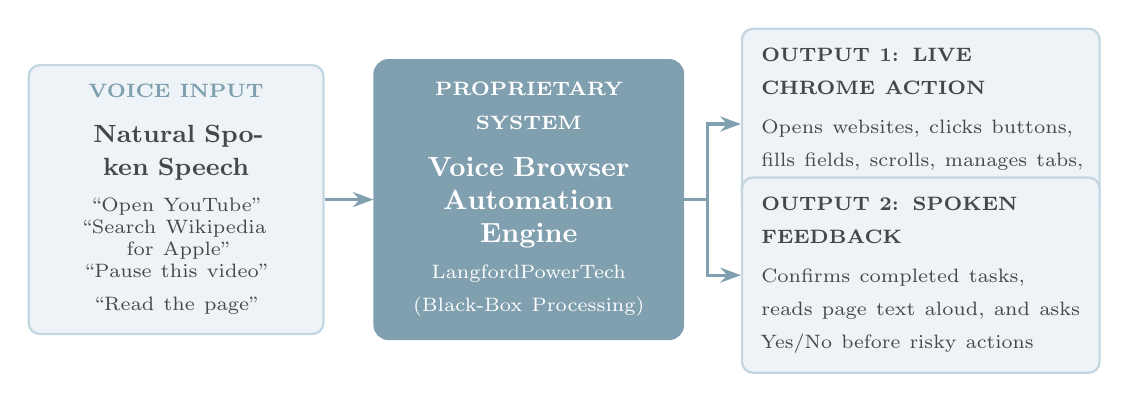
\begin{tikzpicture}[
  inbox/.style={draw=refBorder, fill=refSoft, rounded corners=4pt, line width=0.8pt,
             minimum height=2.35cm, text width=3.25cm, align=center, inner sep=7pt},
  core/.style={draw=refSlate, fill=refSlate, rounded corners=5pt, line width=1pt,
               minimum height=2.55cm, text width=3.35cm, align=center, inner sep=8pt, text=white},
  outbox/.style={draw=refBorder, fill=refSoft, rounded corners=4pt, line width=0.8pt,
                 minimum height=1.18cm, text width=4.05cm, align=left, inner sep=7pt},
  arr/.style={-{Stealth[length=2.6mm,width=1.9mm]}, line width=1.1pt, color=refSlate}
]
  \node[inbox] (input) {%
    {\scriptsize\bfseries\color{refSlate}VOICE INPUT}\\[4pt]
    {\small\bfseries\color{refInk}Natural Spoken Speech}\\[5pt]
    {\scriptsize\color{refInk}``Open YouTube''\\``Search Wikipedia for Apple''\\``Pause this video''\\``Read the page''}
  };

  \node[core, right=0.62cm of input] (engine) {%
    {\scriptsize\textbf{PROPRIETARY SYSTEM}}\\[5pt]
    {\normalsize\bfseries Voice Browser\\Automation Engine}\\[5pt]
    {\scriptsize LangfordPowerTech\\(Black-Box Processing)}
  };

  \node[outbox, right=0.72cm of engine, yshift=0.96cm] (out1) {%
    \raggedright
    {\scriptsize\bfseries\color{refInk}OUTPUT 1: LIVE CHROME ACTION}\\[2pt]
    {\scriptsize\color{refInk}Opens websites, clicks buttons, fills fields, scrolls, manages tabs, and controls media}
  };

  \node[outbox, right=0.72cm of engine, yshift=-0.96cm] (out2) {%
    \raggedright
    {\scriptsize\bfseries\color{refInk}OUTPUT 2: SPOKEN FEEDBACK}\\[2pt]
    {\scriptsize\color{refInk}Confirms completed tasks, reads page text aloud, and asks Yes/No before risky actions}
  };

  \draw[arr] (input.east) -- (engine.west);
  \draw[arr] (engine.east) -- ++(0.30,0) |- (out1.west);
  \draw[arr] (engine.east) -- ++(0.30,0) |- (out2.west);
\end{tikzpicture}
\end{center}

\vspace{0.22cm}
\begin{center}
  {\footnotesize\color{refSlate}\textbf{Key Benefit:} Works directly on the user's regular Google Chrome browser---no custom browser or hand input needed.}
\end{center}
\end{frame}

% =====================================================================
% SLIDE 6: LITERATURE REVIEW (2023 - 2025)
% =====================================================================
\begin{frame}{LITERATURE REVIEW}
\begin{itemize}\setlength{\itemsep}{8pt}\small
  \item \textbf{W3C Web Accessibility Initiative (2023).} \textit{Web Content Accessibility Guidelines (WCAG) 2.2.} World Wide Web Consortium. Defines operability standards for pointer-free and assistive access on modern websites.
  \item \textbf{Deng, X., et al. (2023).} \textit{Mind2Web: Towards a Generalist Agent for the Web.} NeurIPS. Established real-world benchmarks for completing natural-language user tasks across live websites.
  \item \textbf{Zhou, S., et al. (2024).} \textit{WebArena: A Realistic Web Environment for Building Autonomous Agents.} ICLR. Evaluated end-to-end web task completion across shopping, forum, and content workflows, highlighting error-recovery needs.
  \item \textbf{He, H., Yao, W., Ma, K., et al. (2024).} \textit{WebVoyager: Building an End-to-End Web Agent with Large Multimodal Models.} ACL. Demonstrated goal-driven browsing directly on live public websites such as search, travel, and shopping portals.
  \item \textbf{Srinivasan, T., \& Patapati, S. (2025).} \textit{WebNav: An Intelligent Agent for Voice-Controlled Web Navigation.} arXiv:2503.13843. Explored natural-language voice navigation to help users with visual or motor limitations browse websites hands-free.
\end{itemize}
\end{frame}

% =====================================================================
% SLIDE 7: CAPABILITIES 1/2 (SURFING, SEARCH & TABS)
% =====================================================================
\begin{frame}{SYSTEM CAPABILITIES (1/2) --- SURFING \& NAVIGATION}
\renewcommand{\arraystretch}{1.38}
\small
\begin{tabularx}{\textwidth}{@{}p{2.75cm} >{\raggedright\arraybackslash}p{4.65cm} >{\raggedright\arraybackslash}X@{}}
\rowcolor{refSlate}
\textbf{\color{white}Capability} & \textbf{\color{white}Example Voice Input} & \textbf{\color{white}Browser \& Voice Output} \\
\rowcolor{refPage}
\textbf{Open Websites} & ``Open YouTube'', ``Open Google Docs'', ``Open Wikipedia'' & Opens the requested site directly in Chrome and confirms verbally. \\
\rowcolor{refSoft}
\textbf{Direct Search} & ``Search Wikipedia for Apple'', ``Search flights Chennai to Singapore'' & Loads the matching search results directly without typing. \\
\rowcolor{refPage}
\textbf{Tab Control} & ``Open another tab'', ``Switch to previous tab'', ``How many tabs are open?'' & Opens, switches, lists, and closes tabs while keeping Chrome running. \\
\rowcolor{refSoft}
\textbf{Read \& Zoom} & ``Scroll down'', ``Zoom in'', ``Read the page'', ``Explain this'' & Scrolls smoothly, adjusts zoom, and reads clean article text aloud. \\
\rowcolor{refPage}
\textbf{Chained Tasks} & ``Open a new tab and search YouTube for lo-fi'' & Runs multi-step browsing sequences from a single spoken sentence. \\
\hline
\end{tabularx}
\end{frame}

% =====================================================================
% SLIDE 8: CAPABILITIES 2/2 (PAGE & MEDIA CONTROL)
% =====================================================================
\begin{frame}{SYSTEM CAPABILITIES (2/2) --- PAGE \& MEDIA CONTROL}
\renewcommand{\arraystretch}{1.38}
\small
\begin{tabularx}{\textwidth}{@{}p{2.75cm} >{\raggedright\arraybackslash}p{4.65cm} >{\raggedright\arraybackslash}X@{}}
\rowcolor{refSlate}
\textbf{\color{white}Capability} & \textbf{\color{white}Example Voice Input} & \textbf{\color{white}Browser \& Voice Output} \\
\rowcolor{refPage}
\textbf{Page Selection} & ``Select Models'', ``Go to Images'', ``Select Help'' & Clicks visible buttons, links, and section tabs by spoken label. \\
\rowcolor{refSoft}
\textbf{Typing \& Forms} & ``Type\ldots'', ``Press Enter'', ``Next field'' & Enters spoken text into search bars, chat boxes, and web forms. \\
\rowcolor{refPage}
\textbf{Media Control} & ``Pause this video'', ``Volume 35\%'', ``Skip this ad'', ``Speed 1.5x'' & Controls playback, volume, speed, captions, and ads hands-free. \\
\rowcolor{refSoft}
\textbf{Dialogs \& Keys} & ``Close the help window'', ``Dismiss'', ``Control K'' & Closes pop-up overlays and opens quick search boxes cleanly. \\
\rowcolor{refPage}
\textbf{Voice Q\&A} & ``Hey Jarvis, how are you?'' & Answers spoken questions when addressed while ignoring video noise. \\
\hline
\end{tabularx}
\end{frame}

% =====================================================================
% SLIDE 9: SAFETY & ACCESSIBILITY SAFEGUARDS
% =====================================================================
\begin{frame}{SAFETY \& ACCESSIBILITY SAFEGUARDS}
\begin{columns}[T,totalwidth=\textwidth]
  \begin{column}{0.48\textwidth}
    \refcard{1. Verbal Confirmation Gate}{%
      Before sensitive actions (\textbf{Buy, Pay, Submit, Send, Delete, Confirm}), the system pauses and asks: \textit{``I'm about to Send message. Say yes or no.''} Execution continues only after explicit approval.
    }\par\vspace{0.24cm}
    \refcard{3. Last-Tab Protection}{%
      Closing the final tab normally exits Chrome and leaves a hands-free user stranded. The system clears the page to a fresh home screen instead, keeping Chrome open and ready.
    }
  \end{column}
  \begin{column}{0.48\textwidth}
    \refcard{2. Speaker \& Video Noise Filtering}{%
      When watching videos on speakers, dialogue from the video reaches the mic. Smart speech gating ignores ambient commentary so ads or videos never hijack Chrome.
    }\par\vspace{0.24cm}
    \refcard{4. Instant Stop \& Ethical Limits}{%
      Saying \textbf{``Stop''} or \textbf{``Cancel''} halts any running action immediately. Human-verification anti-bot checks (CAPTCHAs) are never bypassed automatically.
    }
  \end{column}
\end{columns}
\end{frame}

% =====================================================================
% SLIDE 10: SAMPLE END-TO-END VOICE SESSION
% =====================================================================
\begin{frame}{SAMPLE END-TO-END VOICE SESSION}
\renewcommand{\arraystretch}{1.28}
\small
\begin{tabularx}{\textwidth}{@{}c >{\raggedright\arraybackslash}p{4.65cm} >{\raggedright\arraybackslash}X@{}}
\rowcolor{refSlate}
\textbf{\color{white}Step} & \textbf{\color{white}User Voice Input} & \textbf{\color{white}Observed Output (Chrome + Voice)} \\
\rowcolor{refPage}
1 & ``Open YouTube'' & Opens YouTube in Chrome; announces \textit{``Opened YouTube.''} \\
\rowcolor{refSoft}
2 & ``Select Spider-Man vs. Ninjas video'' & Opens the matching video; confirms \textit{``Done. Spider-Man vs. Ninjas.''} \\
\rowcolor{refPage}
3 & ``Pause this video'' & Pauses active video playback immediately with zero mouse input. \\
\rowcolor{refSoft}
4 & ``Open another tab'' $\rightarrow$ ``Open Wikipedia'' & Creates a new tab, loads Wikipedia, and confirms verbally. \\
\rowcolor{refPage}
5 & ``Search flights Chennai to Singapore'' & Loads Google flight search results directly in one step. \\
\rowcolor{refSoft}
6 & ``Select Help'' $\rightarrow$ ``Close the help window'' & Opens \textit{Help} and cleanly dismisses the overlay dialog. \\
\rowcolor{refPage}
7 & Sending a message in a web chat app & Pauses: \textit{``I'm about to Send message. Say yes or no.''} $\rightarrow$ User says \textit{``Yes''} $\rightarrow$ Sent safely. \\
\hline
\end{tabularx}
\end{frame}

% =====================================================================
% SLIDE 11: OBSERVED RESULTS & VERIFICATION
% =====================================================================
\begin{frame}{OBSERVED RESULTS \& VERIFICATION}
\begin{columns}[T,totalwidth=\textwidth]
  \begin{column}{0.48\textwidth}
    \refcard{Live Website Coverage}{%
      Verified hands-free across real sites:\\[4pt]
      \textbullet\ \textbf{Media:} YouTube (search, play, pause, skip ad, settings)\\[3pt]
      \textbullet\ \textbf{Knowledge:} Wikipedia, Google Search, Hugging Face\\[3pt]
      \textbullet\ \textbf{Productivity:} Google Docs, AI web chats, multi-tab surfing
    }\par\vspace{0.22cm}
    \refcard{Speaker Noise Resilience}{%
      During live playback of loud gaming and music videos on desktop speakers, video commentary was ignored cleanly with zero unintended clicks.
    }
  \end{column}
  \begin{column}{0.48\textwidth}
    \refcard{User Experience Outcomes}{%
      \textbullet\ \textbf{Fast Everyday Controls:} Scrolling, tab switching, zoom, and playback commands respond immediately.\\[4pt]
      \textbullet\ \textbf{Direct Actions:} Opening sites, searches, and visible links work without manual cursor control.\\[4pt]
      \textbullet\ \textbf{Clear Narration:} Page titles and summaries are spoken cleanly without symbol clutter.
    }\par\vspace{0.22cm}
    \refcard{Safety Verification}{%
      Risky actions (\textit{Buy, Pay, Send, Delete}) reliably paused for verbal Yes/No approval, and Chrome stayed open after closing the last tab.
    }
  \end{column}
\end{columns}
\end{frame}

% =====================================================================
% SLIDE 12: SOCIAL IMPACT & FUTURE SCOPE
% =====================================================================
\begin{frame}{SOCIAL IMPACT \& FUTURE SCOPE}
\begin{columns}[T,totalwidth=\textwidth]
  \begin{column}{0.48\textwidth}
    \refcard{How This System Helps}{%
      \textbullet\ \textbf{Physically Challenged Users:} Restores independent web access for people without hands or with severe motor impairments.\\[6pt]
      \textbullet\ \textbf{Elderly Users:} Replaces small on-screen menus and multi-step clicks with plain spoken requests.\\[6pt]
      \textbullet\ \textbf{Hands-Busy Scenarios:} Supports recovery from temporary hand injuries and hands-free study or work.
    }
  \end{column}
  \begin{column}{0.48\textwidth}
    \refcard{Future Scope}{%
      \textbullet\ \textbf{Regional Language Support:} Add Tamil, Hindi, and mixed-language voice commands for wider reach.\\[6pt]
      \textbullet\ \textbf{Personal Voice Profiles:} Speaker-specific recognition for shared or noisy environments.\\[6pt]
      \textbullet\ \textbf{Custom Voice Routines:} Single-phrase daily routines (e.g., opening morning news, mail, and calendar).
    }
  \end{column}
\end{columns}
\end{frame}

% =====================================================================
% SLIDE 13: QUERIES (Exact Reference Slide 17 Style)
% =====================================================================
\begin{frame}
\vfill
\begin{center}
  {\fontsize{44}{48}\selectfont\color{refInk}Queries?}
\end{center}
\vfill
\end{frame}

% =====================================================================
% SLIDE 14: THANK YOU (Exact Reference Slide 18 Style)
% =====================================================================
\begin{frame}
\vfill
\begin{center}
  {\fontsize{44}{48}\selectfont\color{refInk}Thank You}
\end{center}
\vfill
\end{frame}

\end{document}
